\section{BACKGROUND}\label{background}

We consider the standard partially observable reinforcement learning setting where an agent interacts with an environment $\mathcal{E}$ receiving image observations which do not contain temporal information~\cite{arulkumaran2017brief}. At each time step $t$, the agent receives an observation $s_t$ and selects an action $a_t$ according to a policy $\pi$, which is a mapping from observations to actions. The agent then receives a next observation $s_{t+1}$, a scalar reward $r_t \in \mathbb{R}$, and a Boolean flag $d_t$ indicating whether the agent reached a terminal state. An experience tuple at time $t$ is $(s_t, a_t, s_{t+1}, r_t, d_t)$. A sequence of experience tuples from an initial state to a terminal state is known as a trajectory. The goal of an RL agent is to maximize the total expected cumulative reward at each time step, defined as $R_t = \sum_{k=0}^{\infty} \gamma^{k}r_{t+k}$ for a discount rate $\gamma \in (0,1]$~\cite{mnih2016asynchronous}.

\subsection{Visual-based RL Environments}

The three environments explored in this paper are OpenAI Gym's \texttt{CarRacing-v0}, and the \texttt{take\_cover} and \texttt{defend\_the\_line} scenarios from the ViZDoom platform.

\begin{figure}[h!]
	\centering
	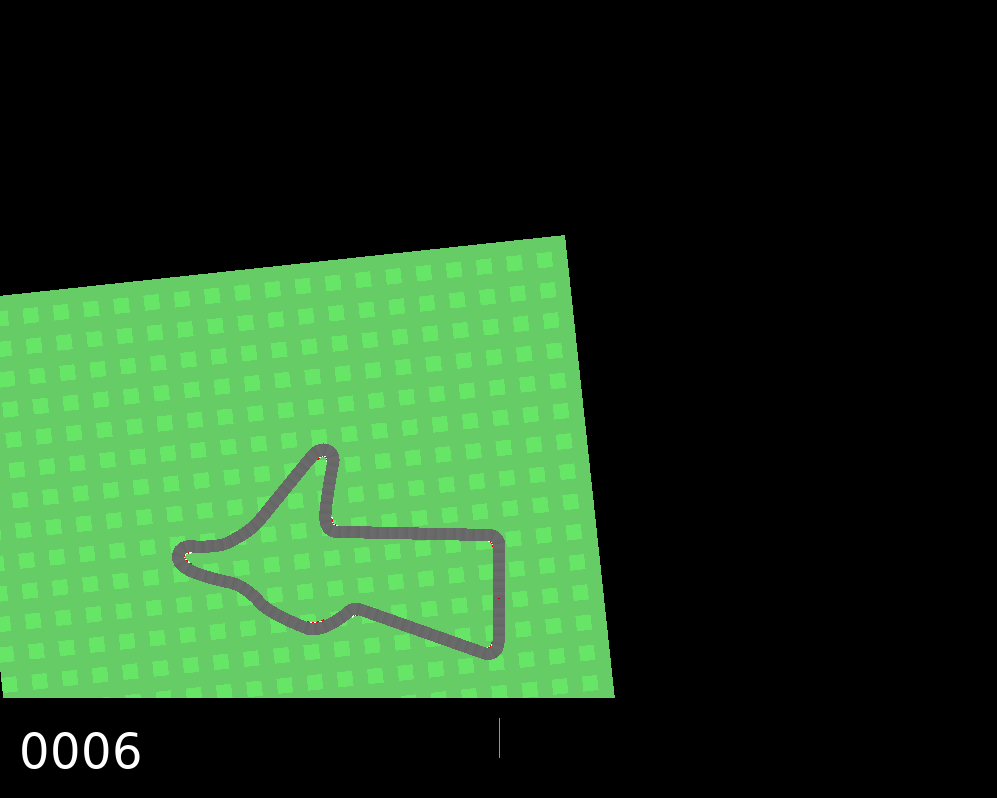
\includegraphics[width=0.15\textwidth]{images/car-map.png}
	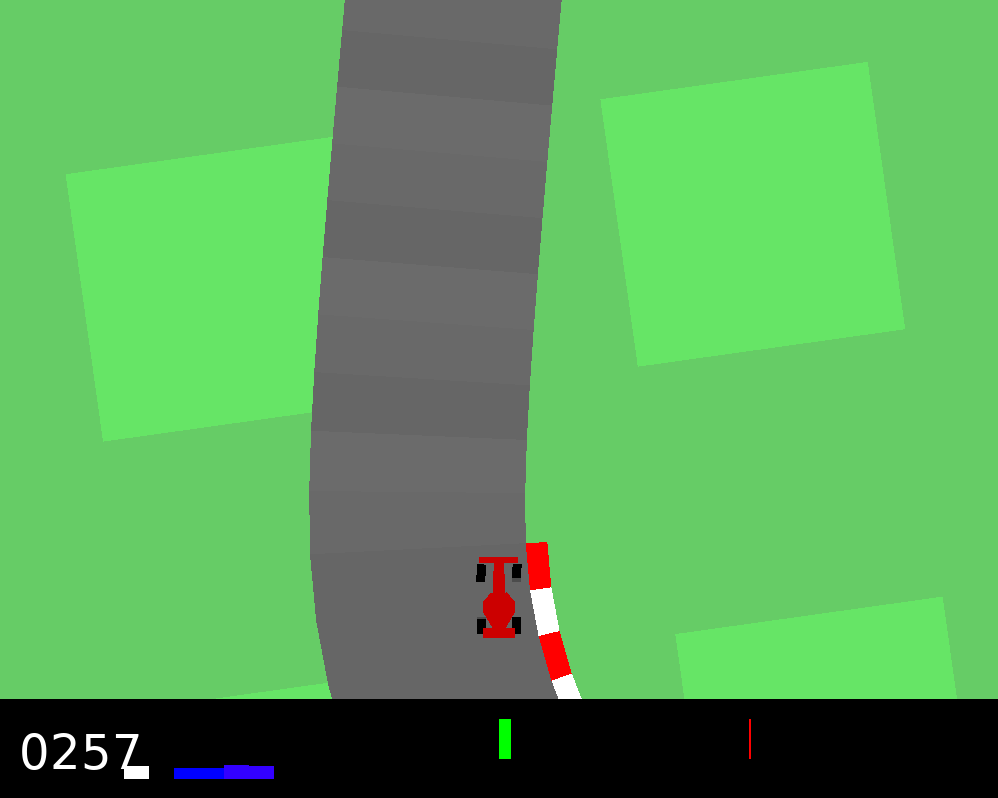
\includegraphics[width=0.15\textwidth]{images/car-tile.png}
	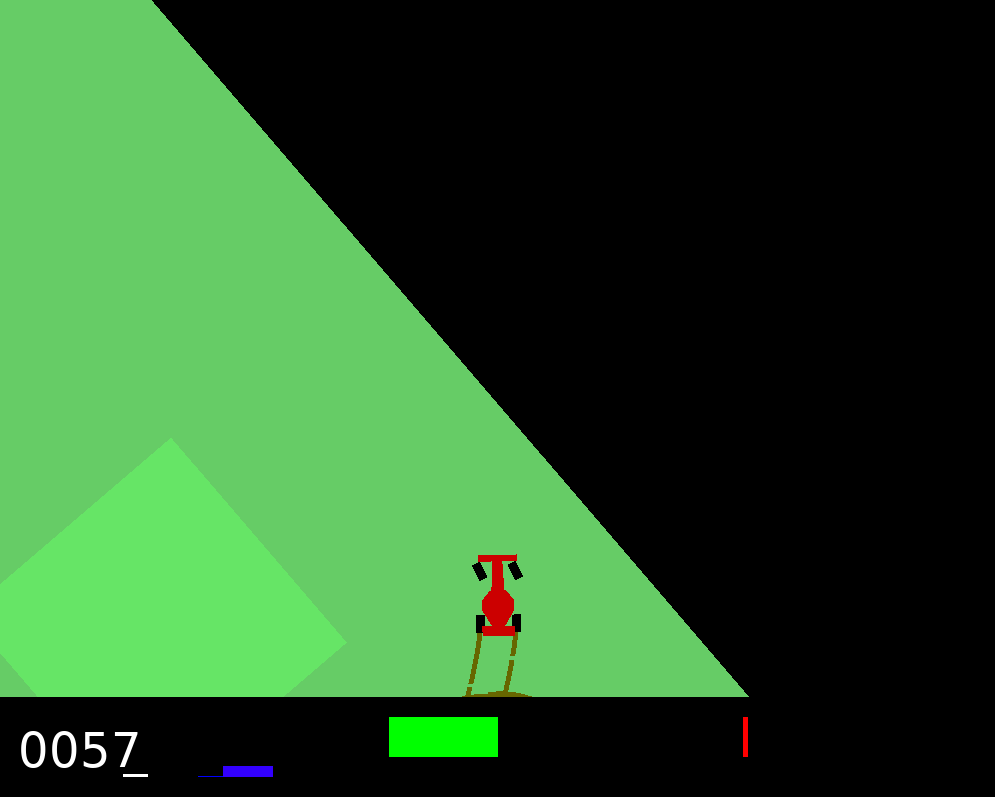
\includegraphics[width=0.15\textwidth]{images/car-die.png}
	\caption{Random Map (left), State Image (middle), Edge of map (right)}\label{fig:carracing}
\end{figure}

\subsubsection{CarRacing-v0}

The \texttt{CarRacing-v0} environment on OpenAI Gym~\cite{brockman2016openai} is a continuous action-space environment where the goal is to control the steering, acceleration, and braking of a car to race it around a randomly generated circuit track in as few time steps as possible. Each observation is an image of the top view of the car on the map as shown in \cref{fig:carracing}. The agent then needs to provide an action consisting of three continuous values for the steering, acceleration, and brake. The track is overlaid with $n$ (usually between $230$ and $320$) rectangular tiles shown in \cref{fig:carracing} (middle) where the agent receives a reward of $1000/n$ upon visiting a tile for the first time. A trajectory terminates after $1000$ time steps, after the agent visits every tile, or after the agent drives off the edge of the map (right of \cref{fig:carracing}). The agent also receives a penalty of $-0.1$ at each time step, encouraging faster completion of the circuit.

\subsubsection{take\_cover and defend\_the\_line}

\begin{figure}[h!]
	\centering
	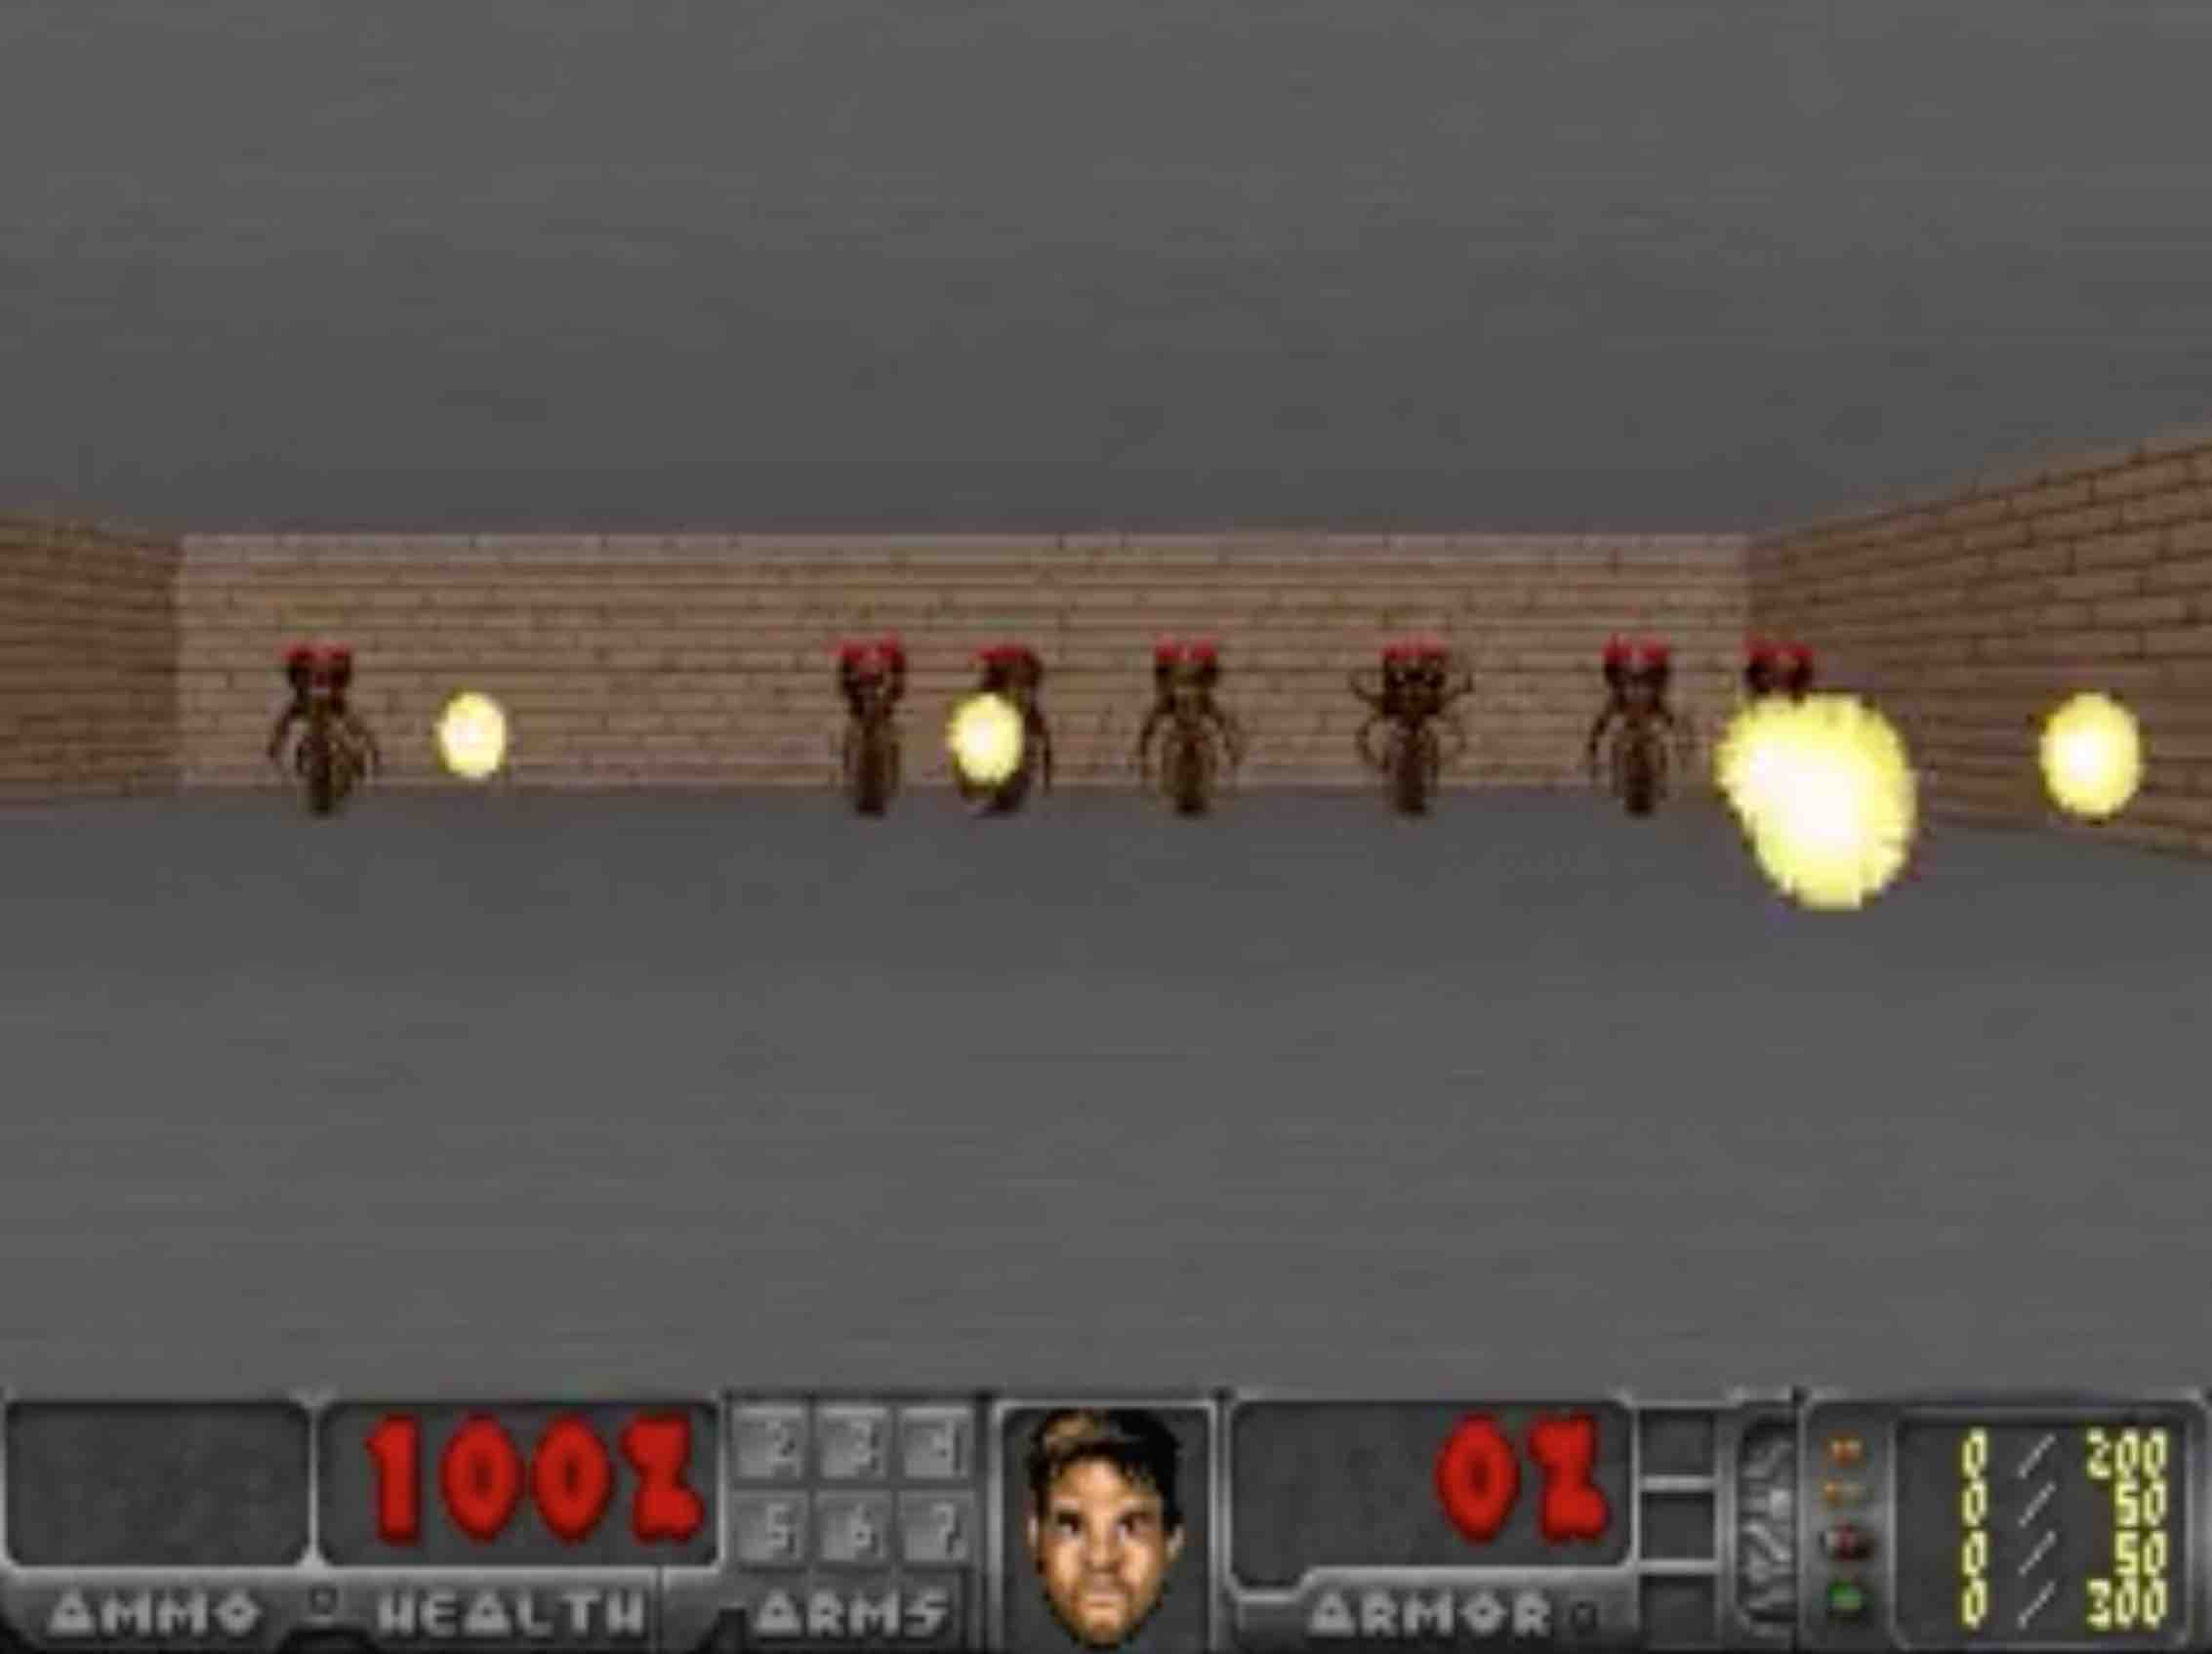
\includegraphics[width=0.23\textwidth]{images/doom2.jpeg}
	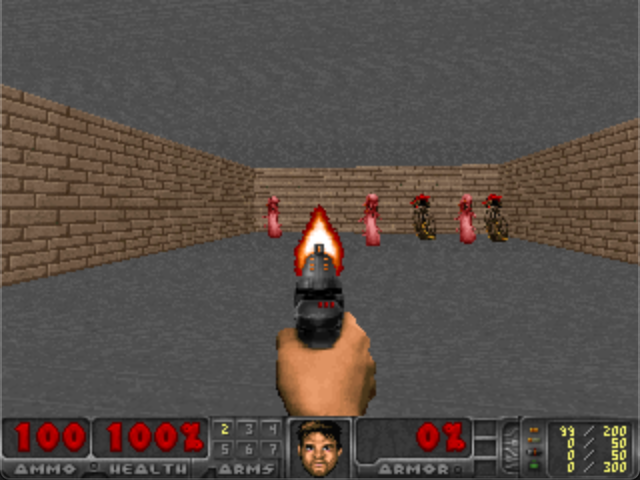
\includegraphics[width=0.23\textwidth]{images/doom1.png}
	\caption{The take_cover (left) and defend_the_line (right) scenarios}\label{fig:doom}
\end{figure}

The scenarios in ViZDoom~\cite{kempka2016vizdoom} are discrete action-space environments where the agent's goal is to survive in a room of monsters. The \texttt{take\_cover} scenario (left of \cref{fig:doom}) requires the agent to select between moving left or right to avoid fireballs launched towards the agent by opposing monsters. The agent receives a reward of $+1$ at every time step where the episode continues until the agent loses all of its health from being hit by fireballs. In the \texttt{defend\_the\_line} environment (right of \cref{fig:doom}), the agent selects between turning left, right or shooting a pistol with limited ammunition straight ahead with the goal of eliminating as many approaching monsters in order to survive. The agent receives $+1$ for each monster eliminated and $-1$ for losing all health from monster attacks.

